\documentclass[11pt]{article}
\usepackage[margin=2.4cm]{geometry}
\usepackage{amsmath,amssymb}
\usepackage{booktabs}
\usepackage{graphicx}
\usepackage{multirow}
\usepackage{caption}
\usepackage[hidelinks]{hyperref}
\captionsetup{font=small,labelfont=bf}
\newcommand{\fcntm}{FC-NTM}
\renewcommand{\thetable}{S\arabic{table}}
\renewcommand{\thefigure}{S\arabic{figure}}
\title{\bfseries Supplementary Material\\[4pt]
\large Auxiliary Experiments, Controls and Metric Definitions}
\author{}
\date{}
\begin{document}
\maketitle

\section{Auxiliary experiments and controls}

\subsection{Long-document truncation control}

The GitHub background field has a long tail (up to 20532 tokens after preprocessing) while the
sentence-embedding baselines truncate at 128 tokens. To check whether the ordering of the main
tables is caused by this truncation, the three baselines were re-run with window pooling: each
document is split into 128-token windows with the model's own tokenizer, the windows are encoded
separately and their vectors averaged, so the embeddings cover the full document; all other
settings are unchanged. Table~\ref{tab:chunked} reports the result.

\begin{table}[t]
\centering
\caption{Long-document control for the sentence-embedding baselines ($C_V$, seeds 11/23/37, mean$\pm$standard deviation). ``Truncated'' encodes only the first 128 tokens (the setting used in the main tables); ``window pooling'' splits a document into 128-token windows with the model's own tokenizer and averages the window vectors, so every token enters exactly one window. Top2Vec uses Doc2Vec document vectors and does not accept window pooling.}
\label{tab:chunked}
\footnotesize
\setlength{\tabcolsep}{3pt}
\begin{tabular}{@{}lcccc@{}}
\toprule
model & GitHub Truncated & GitHub Window pooling & AG News Truncated & AG News Window pooling \\
\midrule
BERTopic & 0.540$\pm$0.015 & 0.582$\pm$0.009 & 0.488$\pm$0.022 & 0.518$\pm$0.011 \\
Top2Vec & 0.493$\pm$0.009 & n/a & 0.498$\pm$0.032 & n/a \\
CombinedTM & 0.643$\pm$0.022 & 0.656$\pm$0.018 & 0.526$\pm$0.037 & 0.488$\pm$0.030 \\
\bottomrule
\end{tabular}
\end{table}

Window pooling raises BERTopic from 0.540 to 0.582 and CombinedTM from 0.643 to 0.656 on GitHub,
and BERTopic from 0.488 to 0.518 while CombinedTM moves from 0.526 to 0.488 on AG News. Even at
their best (GitHub CombinedTM 0.656, AG News BERTopic 0.518) the pooled baselines remain below the
$\beta$ read-out of \fcntm{} (0.701 and 0.586) and well below its class TF--IDF read-out (0.727 and
0.612), so the ordering of bag-of-words models and sentence-embedding baselines is not an artefact
of truncation.

\subsection{Within-corpus length-ratio ladder}

The cross-corpus comparison mixes the length ratio with domain and genre. To separate part of this
confound, the civil corpus is truncated to the first 60 and 30 words of every abstract (length
ratio $11.29\to3.99\to2.02$) and the full, no-cross and no-mask configurations are re-run for the
same 6000/2000 record IDs and the same 7685-word vocabulary (700-epoch budget, all other settings
unchanged). Table~\ref{tab:ladder} reports the result; three observations follow. First, the
$\beta$ read-out of the full model decreases monotonically with truncation
($0.633\to0.595\to0.534$) while the class TF--IDF read-out does not
($0.636\to0.645\to0.606$): the effect of truncation depends on the read-out. Second, the paired
difference of removing cross-field reconstruction does not change monotonically with the length
ratio ($\beta$: $-0.022\to+0.006\to-0.006$; class TF--IDF: $-0.019\to+0.001\to-0.023$). Third, the
cost of removing word masking also fails to follow the ratio ($\beta$: $-0.010\to-0.002\to-0.027$;
class TF--IDF: $-0.011\to-0.017\to-0.025$), and the read-out with the smallest cost differs. Under
a controlled change of the abstract length alone, component importance is therefore neither
monotone in the ratio nor consistent across read-outs, which agrees with the cross-corpus result
that the length ratio is a description rather than a pre-training criterion.

\begin{table}[t]
\centering
\caption{Within-corpus length-ratio ladder on the civil corpus ($K=30$, seeds 11/23/37). $\Delta C_V$ is the paired difference of removing one component relative to the full model (negative means the component matters); parentheses count positive seeds. The length ratio is the mean token ratio of abstracts to titles over the same records and vocabulary.}
\label{tab:ladder}
\small
\setlength{\tabcolsep}{4pt}
\begin{tabular}{@{}llccc@{}}
\toprule
Variant(Length ratio) & read-out & Full $C_V$ & $-\hspace{2pt}$Cross-field recon. $\Delta C_V$
 & $-\hspace{2pt}$Word masking $\Delta C_V$ \\
\midrule
Original(11.29) & $\beta$ & 0.633 & $-$0.022 (0/3) & $-$0.010 (1/3) \\
Original(11.29) & Class TF--IDF & 0.636 & $-$0.019 (0/3) & $-$0.011 (0/3) \\
abs60(3.99) & $\beta$ & 0.595 & $+$0.006 (3/3) & $-$0.002 (2/3) \\
abs60(3.99) & Class TF--IDF & 0.645 & $+$0.001 (1/3) & $-$0.017 (0/3) \\
abs30(2.02) & $\beta$ & 0.534 & $-$0.006 (1/3) & $-$0.027 (0/3) \\
abs30(2.02) & Class TF--IDF & 0.606 & $-$0.023 (0/3) & $-$0.025 (0/3) \\
\bottomrule
\end{tabular}
\end{table}

\subsection{Controls for the occlusion protocol}

Three controls test what the relative degradation can show: (i) a constant unigram model that only
uses training term frequencies and reads no test document; (ii) a shuffled summary, where the
summary of each document is replaced by that of another document while the model is unchanged; and
(iii) the same architecture trained without whole-field dropout. All three use the same masks,
seeds and per-token NLL. Tables~\ref{tab:occl-controls} and~\ref{tab:fielddrop-control} report the
results.

\begin{table}[t]
\centering
\caption{Mechanism controls for the partial-occlusion protocol (seeds 11/23/37). Each cell shows the mean$\pm$standard deviation of the relative degradation $\mathrm{NLL}(100\%)/\mathrm{NLL}(25\%)$ and the absolute NLL at full occlusion. The constant unigram model reads no test input; ``shuffled summary'' replaces each summary by that of another document; ``true summary'' is the main model.}
\label{tab:occl-controls}
\small
\setlength{\tabcolsep}{4pt}
\begin{tabular}{@{}lccc@{}}
\toprule
corpus & constant unigram & shuffled summary(\fcntm{}) & \fcntm{}(true summary) \\
\midrule
GitHub & 0.999$\pm$0.001 / 7.382 & 1.091$\pm$0.002 / 8.567 & 1.029$\pm$0.003 / 7.961 \\
AG News & 1.001$\pm$0.000 / 7.809 & 1.096$\pm$0.001 / 8.622 & 1.018$\pm$0.001 / 7.828 \\
civil corpus & 1.000$\pm$0.001 / 7.875 & 1.084$\pm$0.001 / 8.997 & 1.010$\pm$0.001 / 8.160 \\
\bottomrule
\end{tabular}
\end{table}

\begin{table}[t]
\centering
\caption{Effect of training-time field dropout on the partial-occlusion curve (relative degradation, seeds 11/23/37). The two columns are the same architecture with and without whole-field dropout during training.}
\label{tab:fielddrop-control}
\small
\setlength{\tabcolsep}{4pt}
\begin{tabular}{@{}lcc@{}}
\toprule
corpus & dropout(mainmodel) & No dropout \\
\midrule
GitHub & 1.029$\pm$0.003 & 1.028$\pm$0.007 \\
AG News & 1.018$\pm$0.001 & 1.020$\pm$0.003 \\
civil corpus & 1.010$\pm$0.001 & 1.012$\pm$0.001 \\
\bottomrule
\end{tabular}
\end{table}

Three conclusions follow. First, the constant unigram model has a relative degradation of almost
one on all three corpora (0.999--1.001) and its absolute NLL at full occlusion is lower than that
of \fcntm{} on GitHub and the civil corpus (7.382 versus 7.961 and 7.875 versus 8.160) and close on
AG News (7.809 versus 7.828): a model that reads no test input can be ``stable'' under this ratio,
and the cross-model comparison of absolute likelihood mixes in the calibration of the word
distributions. The ratio is therefore a diagnostic under a specified baseline set, not evidence of
field complementarity by itself. Second, replacing the summary by that of another document raises
the relative degradation from 1.029/1.018/1.010 to 1.091/1.096/1.084 and worsens the absolute NLL
(8.567/8.622/8.997 versus 7.961/7.828/8.160): the model really uses the \emph{content} of the
summary field, which supports ``the summary participates in inference'' more directly than the
ratio itself. Third, removing training-time dropout leaves the ratio almost unchanged
(1.028/1.020/1.012 versus 1.029/1.018/1.010). A same-budget single-encoder control is not
compared under this occlusion protocol, so the behaviour on these curves cannot be attributed
to the two-stream structure alone.

\subsection{Sensitivity of the $\beta$ read-out}

The main tables read $\beta$ from the decoder parameter rows $B_k$, while the document generative
distribution of \fcntm{} is $\operatorname{softmax}(\operatorname{BN}(\theta B))$; the two are not
equivalent. Feeding a unit topic input $e_k$ into the decoder gives the generative distribution,
whose top-10 words overlap the raw read-out with an average Jaccard of only 0.36--0.42 and whose
first word differs for 56\%--74\% of the topics; the $C_V$ and NPMI of the same models also drop
from the raw values (GitHub 0.701$\to$0.625 and 0.233$\to$0.192; AG News 0.586$\to$0.541 and
0.137$\to$0.100; civil corpus 0.633$\to$0.584 and 0.154$\to$0.118), as Table~\ref{tab:beta-readout}
shows. A translation test makes the same point: adding one shared per-word vector to all topic
rows and shifting the BatchNorm running mean leaves the generative distribution pointwise unchanged
(maximum probability difference $\leq5\times10^{-7}$) while 100\% of the raw top-10 lists change.
The class TF--IDF read-out is built from $\theta$ and term counts and is not affected; both
$\beta$ readings are reported, and the generative reading is the one that reflects the model's
generative semantics.

\begin{table}[t]
\centering
\caption{Sensitivity of the $\beta$ read-out (main checkpoints of the three corpora, means over seeds 11/23/37). ``raw'' reads the decoder parameter rows $B_k$; ``BN'' reads the generative distribution $\operatorname{softmax}(\operatorname{BN}(B_k))$ for a unit topic input; Jaccard is the average per-topic overlap of the top-10 words and the top-1 change rate the share of topics whose first word differs.}
\label{tab:beta-readout}
\small
\setlength{\tabcolsep}{4pt}
\begin{tabular}{@{}lcccccc@{}}
\toprule
corpus & raw $C_V$ & BN $C_V$ & raw NPMI & BN NPMI & top-10 Jaccard & top-1 change rate \\
\midrule
GitHub & 0.701 & 0.625 & 0.233 & 0.192 & 0.369 & 0.74 \\
AG News & 0.586 & 0.541 & 0.137 & 0.100 & 0.360 & 0.62 \\
civil corpus & 0.633 & 0.584 & 0.154 & 0.118 & 0.421 & 0.56 \\
\bottomrule
\end{tabular}
\end{table}

\section{Data and metric notes}

\subsection*{Training details of the baselines}

The four baseline families use the following settings. \emph{Gibbs sampling}: BTM is a collapsed
Gibbs sampler over biterms (word pairs within a window of 12 tokens, at most 150 sampled pairs per
document, $\alpha=50/K$, $\beta=0.01$, 300 full sweeps); LDA is fitted by gensim's batch variational
Bayes (50 passes, 120 iterations per pass, symmetric $\alpha$). \emph{Matrix factorisation}: NMF
minimises the Kullback--Leibler divergence between the count matrix and $WH$ with multiplicative
updates (600 iterations, tolerance $10^{-4}$). \emph{Neural variational models}: ProdLDA, ETM,
CTM-lite and FC-NTM share the Adam loop, mini-batch size and budget (700 epochs, 20\% held-out early
stopping); the baselines use learning rate $2\times10^{-3}$ and the main FC-NTM configuration
$5\times10^{-4}$ selected on development data, and the official CombinedTM keeps its own loop
(Adam, learning rate $2\times10^{-3}$, batch size 64, 700 epochs, early stopping on its own held-out
split). \emph{Embedding clustering}: BERTopic runs UMAP followed by HDBSCAN with fixed random
seeds, and Top2Vec fits Doc2Vec document vectors followed by HDBSCAN; both choose their own topic
numbers and are reported for reference only.

\subsection{Data notes}

After stop-word removal and vocabulary filtering, a small number of identical token sequences occur
in both the training and the test split (GitHub 10 records, AG News 8 records, i.e.\ 0.50\% and
0.11\% of the test sets); they come from different original records and are a degeneration of the
filtering rather than duplicated raw records, and the proportion is too small to change the
conclusions. The GitHub background field has a long tail (8501 tokens in the training set and
20532 in the test set after preprocessing) that the sentence-embedding baselines truncate. A few
records have an empty summary after preprocessing (GitHub 6 training and 1 test record; AG News 69
training and 98 test records, up to 1.29\% of the test set); these records are kept in the main
tables with an empty summary input, for which the model has no explicit fallback branch -- the
summary encoder still runs and produces a training-parameter-dependent posterior before gating
with the background posterior (for the seed-11 checkpoint the maximum difference from a
background-only posterior is 0.115 for the GitHub record and 0.261 for the AG News records, with
the most probable topic unchanged in all but three cases). The dropout training and the occlusion
experiments therefore validate \emph{background} absence and should not be extrapolated to missing
summaries. Design iteration used 400 test records (a 1000/400 subsample per corpus); the main text
reports both the full test split and a development-free subset (1600 GitHub and 7200 AG News
records) obtained by exact record-level matching, on which the coherence is recomputed for every
stored model. That re-scoring removes direct overlap only and cannot undo the model and
configuration choices already made, so it is a sensitivity analysis rather than an untouched
confirmation set; an independent confirmation would require repositories or corpora not involved
in the development.

\subsection{Supplementary definitions of the metrics}

$\mathrm{EXCL}_{\mathrm{KADJ}}$ is a $K$-corrected variant of the Bischof--Airoldi exclusivity: the
usual $\mathrm{EXCL}$ is the mean column-normalised mass of the top ten words of each topic, and it
is mapped to $\mathrm{EXCL}_{\mathrm{KADJ}}=(\mathrm{EXCL}-1/K)/(1-1/K)$ so that random topics
score about zero and fully exclusive topics about one. This is our definition rather than the
original measure, and it does not remove the comparability issues between different $K$ or between
different score matrices, so the table only compares models with the same $K=30$. For the
\fcntm{}-cTFIDF rows the value is computed on the class TF--IDF score matrix after row
normalisation, which is not a probability distribution, so those rows are only ranked within the
same read-out and are not compared with $\beta$ rows. IRBO uses the finite-length extrapolated
form, $\mathrm{RBO}_{\mathrm{ext}}=(1-p)\sum_{d=1}^{L}p^{d-1}A_d+p^{L}A_L$ with $p=0.9$, common
depth $L$ and set overlap $A_d$ at depth $d$, and topic diversity is
$\mathrm{IRBO}=1-\overline{\mathrm{RBO}}_{\mathrm{ext}}$. Without the tail term even two identical
ten-word topic lists would obtain a ``similarity'' of $1-p^{L}=0.651$ (diversity 0.349); the bias
varies with the overlap at the final depth (it equals $p^{L}$ for identical and zero for disjoint
lists), so it is not a constant offset shared by all models.

\section{Additional tables and figures}

The table below lists the example topics referenced in the main text.

\begin{table}[t]
\centering
\caption{Example topics on GitHub issues (\fcntm{}, seed 11, $K=30$, best epoch 547 -- the same model as in the main table and figure). The words are generated from the topic--word matrix: the class TF--IDF read-out is computed first and then truncated to the summary and background vocabularies, so no word lies outside the vocabulary; topic names are assigned manually.}
\label{tab:topics}
\footnotesize
\setlength{\tabcolsep}{4pt}
\begin{tabular}{@{}p{2.7cm}p{5.9cm}p{5.9cm}@{}}
\toprule
topics(manual) & Summary-side words(top 10 ) & Background-side words(top 10 ) \\
\midrule
% English translation of topic_table_github_seed11_paper.tex for the
% English supplementary (2026-10-14 review: Chinese labels must not appear).
% T03 (github, seed 11)
Type systems and language services & type typescript function string types regression error property assignable array & type typescript function string types regression error property assignable array \\  % label=typescript mass=0.069
% T08 (github, seed 11)
DuckDB build and distribution & duckdb all python data sets distribution architecture linux required nightly & duckdb all python data reproducing sets distribution architecture linux required \\  % label=duckdb mass=0.055
% T05 (github, seed 11)
Redis replication and clustering & master cluster redis node sentinel slave nodes docker failover command & master cluster redis node sentinel slave nodes docker failover command \\  % label=redis mass=0.035
% T07 (github, seed 11)
Configuration and command semantics & redis command key set value some keys error one cluster & redis command key set value some keys error one cluster \\  % label=redis mass=0.050
% T09 (github, seed 11)
Language feature proposals & javascript type typescript suggestion types existing runtime change feature syntax & javascript type typescript suggestion types wouldn existing runtime change feature \\  % label=typescript mass=0.043
% T02 (github, seed 11)
Event loop and cache metrics & idle addr sub flags cmd age multi free events name & qbuf psub oll obl idle addr sub flags cmd omem   % label=redis mass=0.007

\\   % the row terminator lives here, not in the \input file: a trailing \\
     % at the end of an \input-ed file breaks \bottomrule (Misplaced \noalign)
\bottomrule
\end{tabular}
\end{table}

\subsection{Civil topic case studies}

The table below lists four readable topics of the seed-11 civil model with one representative
record each, plus two failure cases found by scanning the labelled test records. In the first
failure case a seismicity paper is routed by its title alone to the BIM topic, and the abstract
restores the correct label; in the second, an entry whose title mentions corrosion is routed by
both settings to the related ``concrete reinforcement materials'' topic instead of the corrosion
topic. Routing uses the same majority-vote mapping protocol as the main archival task. The
representative records of the four topics are selected by topic mass on the training split and
are not held-out evidence; the two failure cases are test records. The mixed laboratory-materials
topic is an interpretability problem (mixed vocabularies), not a routing failure --- its
representative record is routed correctly.

\begin{table}[t]
\centering
\caption{Case studies on the civil corpus (\fcntm{}, seed 11, $\beta$ read-out; ``title-only'' and ``full-field'' give the routing decision of the same mapping protocol, and ``miss'' marks a decision different from the OpenAlex label; OpenAlex Work IDs are given in parentheses).}
\label{tab:civil-cases}
\scriptsize
\setlength{\tabcolsep}{3pt}
\begin{tabular}{@{}p{2.6cm}p{4.0cm}p{3.6cm}p{2.4cm}cc@{}}
\toprule
Topic(manual) & Top words($\beta$ read-out) & Representative record & OpenAlex label & title-only & full-field \\
\midrule
Asphalt mixture design and performance & asphalt, mixture, binder, mixtures, temperature, test, performance, modified, stability, low & Synergetic Effect of NanoZnO and Trinidad Lake Asphalt for Antiaging Properties of SBSModified Asphalt (W3007633598) & Asphalt Pavement Performance Evaluation & correct & correct \\
Seismic response of tunnels and piles & response, ground, motion, seismic, tunnel, earthquake, acceleration, foundation, pile, wave & Earthquake ground-motion parameters at stiff sites in Addis Ababa, Ethiopia (W2033407901) & Seismic Performance and Analysis & correct & correct \\
BIM and construction management & construction, information, bim, building, project, industry, management, projects, implementation, process & Exploring the Adoption of Building Information Modeling (BIM) in the Jordanian Construction Industry (W2624290857) & BIM and Construction Integration & correct & correct \\
Structural mechanics: shear, buckling, composite beams & load, capacity, finite, element, shear, beam, plate, composite, behavior, buckling & Out-of-Plane Secondary Bifurcation Buckling Behavior of Elastic Circle Pipe Arch (W2063862378) & Structural Load-Bearing Analysis & correct & correct \\
Mixed laboratory-materials topic (failure case) & diamond, wood, metal, cell, density, wear, segments, adsorption, matrix, saw & Pseudotsuga menziesii (Mirb.) Franco wood basic density in the Patagonia Argentina (W1511725581) & Wood Treatment and Properties & correct & correct \\
Failure case: title-only misrouted & construction, information, bim, building, project, industry, management, projects, implementation, process & United States building code approach to variations in regional seismicity (W2525447080) & Seismic Performance and Analysis & miss & correct \\
Failure case: title-only misrouted & strength, fiber, steel, concrete, mechanical, reinforced, fibers, specimens, compressive, tensile & Corrosion Behavior of Reinforcing steel in Concrete (W4387417777) & Concrete Corrosion and Durability & miss & miss \\

\\   % the row terminator lives here, not in the \input file
\bottomrule
\end{tabular}
\end{table}

\section{Ablations and secondary comparisons}

Tables S8--S13 collect the ablations and secondary comparisons that the main manuscript cites to
this supplement: the field-redundancy measures, the field-restricted read-out comparison, the
three-step fusion ablation, the core-component ablation, the sensitivity to the
fusion-reconstruction weight, and the whole-field occlusion diagnostic. All tables use the same
protocol, vocabulary and read-out definitions as the main-text tables.

\begin{table}[t]
\centering
\caption{Field redundancy, measured occlusion gap and the $C_V$ difference against BTM on two corpora. Redundancy is fitted on the training split and evaluated on the test split and includes constructive controls (exact copy $=1.000$, cross-document shuffle $\approx0.000$); the occlusion $\Delta C_V$ is the mean$\pm$standard deviation over seeds 11/23/37 with dropout training. The last column gives the $C_V$ difference under the matched class TF--IDF read-out and under BTM's native $\beta$ read-out.}
\label{tab:conditional}
\footnotesize
\setlength{\tabcolsep}{4pt}
\begin{tabular}{@{}lcccc@{}}
\toprule
Corpus & Held-out Ridge $R^2$ & Held-out $\rho^2_{\mathrm{cca}}$
 & Occlusion $\Delta C_V$ & $C_V$ gap, cTFIDF$-$BTM (matched / $\beta$) \\
\midrule
GitHub issues & 0.230 & 0.306 & $+$0.009$\pm$0.022 & $+$0.027 / $+$0.014 \\
AG News & 0.158 & 0.245 & $+$0.018$\pm$0.013 & $+$0.019 / $+$0.012 \\
\bottomrule
\end{tabular}
\end{table}

\begin{table}[t]
\centering
\caption{Field-restricted read-out ($C_V$, mean$\pm$standard deviation over seeds 11/23/37). Every topic--word matrix is truncated to the vocabulary of one field and scored against that field's test text only; ``background view'' is the abstract/body side and ``summary view'' the title side. FC-NTM's summary view is scored on 20--22 scorable topics per seed on GitHub (29--30 on AG News, 26--28 on the civil corpus) because topics whose ten field words never occur in the held-out text get an undefined $C_V$.}
\label{tab:fieldview-baselines}
\small
\setlength{\tabcolsep}{4pt}
\begin{tabular}{@{}llcc@{}}
\toprule
Corpus & Model & Background view $C_V$ & Summary view $C_V$ \\
\midrule
\multirow{5}{*}{GitHub issues}
 & \fcntm{} & 0.697$\pm$0.016 & 0.426$\pm$0.012 \\
 & BTM & \textbf{0.710$\pm$0.011} & 0.396$\pm$0.018 \\
 & NMF & 0.609$\pm$0.004 & 0.433$\pm$0.002 \\
 & LDA & 0.543$\pm$0.011 & 0.466$\pm$0.005 \\
 & ProdLDA & 0.575$\pm$0.006 & \textbf{0.467$\pm$0.034} \\
\midrule
\multirow{5}{*}{AG News}
 & \fcntm{} & 0.566$\pm$0.016 & 0.423$\pm$0.015 \\
 & BTM & \textbf{0.586$\pm$0.015} & 0.399$\pm$0.018 \\
 & NMF & 0.477$\pm$0.015 & 0.444$\pm$0.002 \\
 & LDA & 0.419$\pm$0.007 & \textbf{0.486$\pm$0.006} \\
 & ProdLDA & 0.499$\pm$0.032 & 0.438$\pm$0.007 \\
\midrule
\multirow{5}{*}{Civil corpus}
 & \fcntm{} & \textbf{0.637$\pm$0.015} & 0.408$\pm$0.005 \\
 & BTM & 0.589$\pm$0.014 & 0.382$\pm$0.008 \\
 & NMF & 0.600$\pm$0.009 & 0.398$\pm$0.013 \\
 & LDA & 0.554$\pm$0.008 & 0.415$\pm$0.006 \\
 & ProdLDA & 0.576$\pm$0.025 & \textbf{0.419$\pm$0.012} \\
\bottomrule
\end{tabular}
\end{table}

\begin{table}[t]
\centering
\caption{Three-step fusion ablation on GitHub issues ($K=30$, seeds 11/23/37, same protocol). Within one read-out each row changes exactly one thing: first the fused mixture $\theta_{\mathrm{fuse}}$ is decoded into the reconstruction term (mean fusion), then mean fusion is replaced by a learnable gate (the main model). ``Positive pairs'' counts the seeds whose paired difference against the row above is positive ($C_V$, NPMI).}
\label{tab:fusion}
\small
\begin{tabular}{llcccc}
\toprule
Read-out & Configuration & $C_V$ & NPMI & Positive pairs & UMass \\
\midrule
\multirow{3}{*}{$\beta$} & No fusion & 0.721$\pm$0.016 & 0.266$\pm$0.012 & --- & $-$2.63 \\
 & Mean fusion + fusion recon. & 0.708$\pm$0.016 & 0.245$\pm$0.013 & 1/3, 0/3 & $-$2.98 \\
 & Gated fusion (main model) & 0.701$\pm$0.016 & 0.233$\pm$0.012 & 0/3, 0/3 & $-$3.16 \\
\midrule
\multirow{3}{*}{cTFIDF} & No fusion & 0.714$\pm$0.001 & 0.262$\pm$0.007 & --- & $-$1.86 \\
 & Mean fusion + fusion recon. & 0.728$\pm$0.007 & 0.275$\pm$0.015 & 3/3, 3/3 & $-$1.91 \\
 & Gated fusion (main model) & 0.727$\pm$0.022 & 0.274$\pm$0.026 & 1/3, 1/3 & $-$1.90 \\
\bottomrule
\end{tabular}
\end{table}

\begin{table}[t]
\centering
\caption{Core-component ablation on three corpora and two read-outs ($K=30$, seeds 11/23/37, 700-epoch budget, all other settings identical to the main model). Each column switches off one component: cross-field reconstruction of both streams, the JS consistency weight, field-level word masking, and whole-field dropout; the fusion-reconstruction term is kept in all columns. Values are mean paired $\Delta C_V$ (negative means the component matters), parentheses count positive pairs.}
\label{tab:core-ablation}
\small
\setlength{\tabcolsep}{5pt}
\begin{tabular}{llcccc}
\toprule
Corpus & Read-out & $-$Cross-field recon. & $-$JS consistency & $-$Word masking & $-$Field dropout \\
\midrule
GitHub & $\beta$ & $+$0.021 (2/3) & $-$0.001 (1/3) & $-$0.012 (1/3) & $-$0.023 (1/3) \\
GitHub & Class TF-IDF & $-$0.005 (1/3) & $+$0.004 (2/3) & $-$0.004 (1/3) & $-$0.021 (1/3) \\
\midrule
AG News & $\beta$ & $-$0.011 (2/3) & $+$0.003 (1/3) & $-$0.026 (0/3) & $-$0.010 (1/3) \\
AG News & Class TF-IDF & $-$0.022 (0/3) & $-$0.002 (1/3) & $-$0.043 (0/3) & $-$0.023 (1/3) \\
\midrule
Civil corpus & $\beta$ & $-$0.022 (0/3) & $+$0.001 (2/3) & $-$0.010 (1/3) & $+$0.001 (1/3) \\
Civil corpus & Class TF-IDF & $-$0.019 (0/3) & $-$0.002 (0/3) & $-$0.012 (0/3) & $-$0.034 (0/3) \\
\bottomrule
\end{tabular}
\end{table}

\begin{table}[t]
\centering
\caption{Sensitivity to the fusion-reconstruction weight $\lambda_f$ on GitHub issues (gated fusion, seeds 11/23/37). $\lambda_f=0$ is the no-fusion setting, $\lambda_f=0.5$ is the value used throughout; all other settings match the main model.}
\label{tab:weight}
\small
\setlength{\tabcolsep}{4pt}
\begin{tabular}{lcccc}
\toprule
\multirow{2}{*}{$\lambda_f$} & \multicolumn{2}{c}{$\beta$ read-out} & \multicolumn{2}{c}{Class TF--IDF} \\
 & $C_V$ & NPMI & $C_V$ & NPMI \\
\midrule
0 & 0.721$\pm$0.016 & 0.266$\pm$0.012 & 0.714$\pm$0.001 & 0.262$\pm$0.007 \\
0.25 & 0.697$\pm$0.015 & 0.217$\pm$0.031 & 0.713$\pm$0.015 & 0.262$\pm$0.004 \\
0.5 & 0.701$\pm$0.016 & 0.233$\pm$0.012 & 0.727$\pm$0.022 & 0.274$\pm$0.026 \\
1.0 & 0.716$\pm$0.012 & 0.246$\pm$0.026 & 0.723$\pm$0.012 & 0.277$\pm$0.018 \\
\bottomrule
\end{tabular}
\end{table}

\begin{table}[t]
\centering
\caption{Whole-field occlusion at inference time ($K=30$, final configuration, 700-epoch budget). $\Delta C_V$ is the coherence difference between full-field and occluded inference under the same read-out; $\Delta\mathrm{NLL}$ is the per-token increase; agreement is the fraction of documents whose most probable topic is unchanged. The two rows of a corpus use the same seeds, isolating the effect of the training-time dropout setting.}
\label{tab:occlusion}
\small
\setlength{\tabcolsep}{4pt}
\begin{tabular}{llcccccc}
\toprule
Corpus & Training setting & $C_V^{\mathrm{full}}$ & $C_V^{\mathrm{occ}}$ & $\Delta C_V$
 & $\Delta\mathrm{NLL}$(per token) & Agreement & Mean JS \\
\midrule
GitHub & Dropout ($p=0.5$) & 0.727 & 0.717 & $+$0.009 & $+$0.241 & 0.345 & 0.082 \\
       & No dropout & 0.705 & 0.725 & $-$0.020 & $+$0.242 & 0.346 & 0.092 \\
\midrule
Civil corpus & Dropout ($p=0.5$) & 0.636 & 0.627 & $+$0.009 & $+$0.103 & 0.673 & 0.033 \\
        & No dropout & 0.602 & 0.597 & $+$0.005 & $+$0.125 & 0.642 & 0.039 \\
\midrule
AG News & Dropout ($p=0.5$) & 0.612 & 0.594 & $+$0.018 & $+$0.232 & 0.520 & 0.049 \\
        & No dropout & 0.589 & 0.582 & $+$0.007 & $+$0.269 & 0.498 & 0.060 \\
\bottomrule
\end{tabular}
\end{table}

\section{Extended results}

Tables S14--S20 and Figures S1--S3 collect the cross-corpus, occlusion,
read-out and application results that the shortened manuscript cites to this
supplement. They use the same protocol, vocabulary and read-outs as the
main-text tables.

\begin{table}[t]
\centering
\caption{Topic quality on AG News (unified evaluation vocabulary, ten words per topic; values are means over seeds 11/23/37 where applicable, and the training procedure differs across algorithm families as described in the main text; BERTopic and Top2Vec choose their own topic numbers and are shown for reference).}
\label{tab:agnews}
\small
\begin{tabular}{lcccccc}
\toprule
Model & Topics & $C_V$ & NPMI & UMass & EXCL$_{\mathrm{KADJ}}$ & IRBO \\
\midrule
BTM & 30 & 0.600$\pm$0.011 & 0.164$\pm$0.005 & $-$4.19 & 0.409 & 0.980 \\
CombinedTM & 30 & 0.526$\pm$0.037 & 0.057$\pm$0.070 & $-$8.01 & 0.118 & 1.000 \\
\fcntm{}-cTFIDF & 30 & \textbf{0.612}$\pm$0.014 & \textbf{0.173}$\pm$0.012 & $-$4.20 & 0.193 & 0.974 \\
\fcntm{} & 30 & 0.586$\pm$0.026 & 0.137$\pm$0.022 & $-$4.91 & 0.013 & 0.993 \\
ETM & 30 & 0.506$\pm$0.014 & 0.092$\pm$0.010 & $-$5.12 & 0.439 & 0.982 \\
ProdLDA & 30 & 0.526$\pm$0.031 & 0.071$\pm$0.015 & $-$6.61 & 0.055 & 0.999 \\
Top2Vec & 2.7 & 0.498$\pm$0.032 & 0.099$\pm$0.031 & $-$2.92 & 0.268 & 0.937 \\
NMF & 30 & 0.494$\pm$0.015 & 0.069$\pm$0.013 & $-$5.96 & 0.799 & 0.997 \\
BERTopic & 29 & 0.488$\pm$0.022 & 0.035$\pm$0.026 & $-$8.81 & 0.681 & 0.997 \\
CTM-lite & 30 & 0.431$\pm$0.023 & $-$0.015$\pm$0.016 & $-$8.34 & 0.041 & 0.998 \\
LDA & 30 & 0.421$\pm$0.013 & $-$0.066$\pm$0.018 & $-$8.62 & 0.696 & 0.994 \\
\bottomrule
\end{tabular}
\end{table}

\begin{table}[t]
\centering
\caption{Topic quality on GitHub issues (same evaluation protocol and read-outs as Table~\ref{tab:agnews}; the FC-NTM rows, BTM, ETM, CombinedTM, ProdLDA and CTM-lite are three-seed results).}
\label{tab:github}
\small
\begin{tabular}{lcccccc}
\toprule
Model & Topics & $C_V$ & NPMI & UMass & EXCL$_{\mathrm{KADJ}}$ & IRBO \\
\midrule
BTM & 30 & 0.712$\pm$0.012 & 0.232$\pm$0.012 & $-$1.79 & 0.349 & 0.934 \\
\fcntm{}-cTFIDF & 30 & \textbf{0.727}$\pm$0.022 & \textbf{0.274}$\pm$0.026 & $-$1.90 & 0.133 & 0.901 \\
\fcntm{} & 30 & 0.701$\pm$0.016 & 0.233$\pm$0.012 & $-$3.16 & 0.010 & 0.967 \\
ETM & 30 & 0.675$\pm$0.014 & 0.213$\pm$0.010 & $-$2.14 & 0.366 & 0.955 \\
CombinedTM & 30 & 0.643$\pm$0.022 & 0.193$\pm$0.015 & $-$4.70 & 0.031 & 0.983 \\
NMF & 30 & 0.614$\pm$0.005 & 0.164$\pm$0.003 & $-$3.26 & 0.595 & 0.985 \\
ProdLDA & 30 & 0.579$\pm$0.007 & 0.107$\pm$0.012 & $-$5.21 & 0.043 & 0.995 \\
CTM-lite & 30 & 0.585$\pm$0.032 & 0.129$\pm$0.036 & $-$5.11 & 0.011 & 0.989 \\
LDA & 30 & 0.546$\pm$0.011 & 0.074$\pm$0.017 & $-$4.21 & 0.684 & 0.990 \\
BERTopic & 29 & 0.540$\pm$0.015 & 0.076$\pm$0.012 & $-$7.00 & 0.546 & 0.976 \\
Top2Vec & 160 & 0.493$\pm$0.009 & $-$0.008$\pm$0.013 & $-$9.65 & 0.337 & 0.994 \\
\bottomrule
\end{tabular}
\end{table}

\begin{table}[t]
\centering
\caption{Read-out comparison ($K=30$, means over seeds 11/23/37). Each model is first read out through its own topic--word matrix ($\beta$ read-out) and then through a class TF--IDF read-out aggregated from its training-set posterior $\theta$; BTM enters the same read-out through the point-estimate document--topic posterior of its original Section 3.3, and the FC-NTM row is the same model as in Tables~\ref{tab:agnews} and~\ref{tab:github}.}
\label{tab:fair}
\footnotesize
\setlength{\tabcolsep}{4pt}
\begin{tabular}{@{}llcc@{}}
\toprule
Corpus & Model & $\beta$ read-out $C_V$ / NPMI & Class TF--IDF $C_V$ / NPMI \\
\midrule
 \multirow{7}{*}{GitHub}
 & \fcntm{}(3 seed mean) & 0.701 / 0.233 & \textbf{0.727 / 0.274} \\
 & ETM & 0.675 / 0.213 & 0.669 / 0.220 \\
 & ProdLDA & 0.579 / 0.107 & 0.666 / 0.215 \\
 & CTM-lite & 0.585 / 0.129 & 0.675 / 0.216 \\
 & NMF & 0.614 / 0.164 & 0.603 / 0.158 \\
 & LDA & 0.546 / 0.074 & 0.614 / 0.193 \\
 & BTM(3 seeds) & 0.712 / 0.232 & 0.700 / 0.235 \\
\midrule
 \multirow{7}{*}{AG News}
 & \fcntm{}(3 seed mean) & 0.586 / 0.137 & \textbf{0.612 / 0.173} \\
 & ProdLDA & 0.526 / 0.071 & 0.544 / 0.125 \\
 & NMF & 0.494 / 0.069 & 0.539 / 0.121 \\
 & ETM & 0.506 / 0.092 & 0.511 / 0.082 \\
 & CTM-lite & 0.431 / $-$0.015 & 0.455 / 0.062 \\
 & LDA & 0.421 / $-$0.066 & 0.451 / 0.010 \\
 & BTM(3 seeds) & 0.600 / 0.164 & 0.593 / 0.169 \\
\midrule
 \multirow{7}{*}{Civil corpus}
 & \fcntm{}(3 seed mean) & \textbf{0.633 / 0.154} & \textbf{0.636 / 0.159} \\
 & NMF & 0.598 / 0.135 & 0.607 / 0.142 \\
 & ETM & 0.581 / 0.119 & 0.603 / 0.134 \\
 & BTM(3 seeds) & 0.583 / 0.128 & 0.590 / 0.139 \\
 & LDA & 0.554 / 0.056 & 0.575 / 0.105 \\
 & ProdLDA & 0.580 / 0.125 & 0.545 / 0.108 \\
 & CTM-lite & 0.536 / 0.098 & 0.530 / 0.094 \\
\bottomrule
\end{tabular}
\end{table}

\begin{table}[t]
\centering
\caption{Partial-occlusion curves on GitHub issues (seed 11). NLL is the per-token negative log-likelihood of the occluded tokens (lower is better); relative degradation is $\mathrm{NLL}(100\%)/\mathrm{NLL}(25\%)$; agreement is the fraction of documents holding their most probable topic at 100\% occlusion. BTM enters through its document--topic posterior.}
\label{tab:occl-robust}
\footnotesize
\setlength{\tabcolsep}{3pt}
\begin{tabular}{@{}lccccc@{}}
\toprule
Model & NLL(25\%) & NLL(50\%) & NLL(75\%) & NLL(100\%) & Degradation / Agreement \\
\midrule
\fcntm{} & 7.712 & 7.735 & 7.790 & 7.960 & \textbf{1.032} / 0.358 \\
LDA & 6.802 & 6.854 & 6.948 & 7.302 & 1.074 / 0.420 \\
ProdLDA & 7.558 & 7.588 & 7.668 & 8.165 & 1.080 / 0.354 \\
BTM & 6.630 & 6.639 & 6.670 & \textbf{6.972} & 1.052 / 0.448 \\
ETM & \textbf{6.616} & 6.643 & 6.708 & 7.202 & 1.089 / 0.452 \\
NMF & 6.972 & 7.169 & 7.561 & 10.255 & 1.471 / \textbf{0.469} \\
\bottomrule
\end{tabular}
\end{table}

\begin{table}[t]
\centering
\caption{Partial-occlusion behaviour on the three corpora (seeds 11/23/37, mean$\pm$standard deviation; the mask is redrawn per seed). Bold marks the smallest relative degradation per corpus. Field asymmetry is described by the mean background/summary token ratio and by the token-type share of background words that do not occur in the summary of the same document.}
\label{tab:occl-cross}
\footnotesize
\setlength{\tabcolsep}{3pt}
\begin{tabular}{@{}llcc@{}}
\toprule
Corpus(Field asymmetry) & Model & Relative degradation & Agreement(100\%) \\
\midrule
\multirow{6}{*}{\shortstack[l]{GitHub issues\\ Length ratio 12.9\\ Background-exclusive 0.877}}
 & \fcntm{} & \textbf{1.029$\pm$0.003} & 0.345 \\
 & LDA & 1.074$\pm$0.000 & 0.424 \\
 & ProdLDA & 1.081$\pm$0.002 & 0.347 \\
 & ETM & 1.088$\pm$0.003 & 0.455 \\
 & BTM & 1.052$\pm$0.001 & 0.438 \\
 & NMF & 1.470$\pm$0.006 & 0.467 \\
\midrule
\multirow{6}{*}{\shortstack[l]{Civil corpus\\ Length ratio 11.2\\ Background-exclusive 0.894}}
 & \fcntm{} & 1.010$\pm$0.001 & 0.673 \\
 & LDA & 1.036$\pm$0.002 & 0.561 \\
 & ProdLDA & 1.027$\pm$0.003 & 0.552 \\
 & ETM & 1.041$\pm$0.001 & 0.655 \\
 & BTM & \textbf{1.007$\pm$0.001} & 0.561 \\
 & NMF & 1.173$\pm$0.001 & 0.655 \\
\midrule
\multirow{6}{*}{\shortstack[l]{AG News\\ Length ratio 3.9\\ Background-exclusive 0.868}}
 & \fcntm{} & 1.018$\pm$0.001 & 0.520 \\
 & LDA & \textbf{1.005$\pm$0.001} & 0.436 \\
 & ProdLDA & 1.026$\pm$0.001 & 0.489 \\
 & ETM & 1.072$\pm$0.001 & 0.554 \\
 & BTM & 1.044$\pm$0.001 & 0.555 \\
 & NMF & 1.408$\pm$0.003 & 0.546 \\
\bottomrule
\end{tabular}
\end{table}

\begin{table}[t]
\centering
\caption{Concatenated-field single-encoder control (seeds 11/23/37; same budget, vocabulary and read-outs). $\Delta$ is \fcntm{} minus the control, with positive pairs in parentheses.}
\label{tab:concat}
\small
\begin{tabular}{llcccc}
\toprule
Corpus & Read-out & \fcntm{} & Concatenated & $\Delta$ (positive pairs) \\
\midrule
GitHub & $\beta$ & 0.701$\pm$0.016 & 0.683$\pm$0.014 & $+$0.017 (2/3) \\
GitHub & Class TF--IDF & 0.727$\pm$0.022 & 0.710$\pm$0.020 & $+$0.017 (1/3) \\
AG News & $\beta$ & 0.586$\pm$0.026 & 0.574$\pm$0.019 & $+$0.012 (2/3) \\
AG News & Class TF--IDF & 0.612$\pm$0.014 & 0.584$\pm$0.009 & $+$0.028 (3/3) \\
Civil corpus & $\beta$ & 0.633$\pm$0.014 & 0.623$\pm$0.014 & $+$0.010 (2/3) \\
Civil corpus & Class TF--IDF & 0.636$\pm$0.014 & 0.606$\pm$0.014 & $+$0.029 (2/3) \\
\bottomrule
\end{tabular}
\end{table}

\begin{table}[t]
\centering
\caption{Title-only routing to the 15 most frequent OpenAlex topics of the civil corpus (seeds 11/23/37; 857 test records, coverage 42.9\%). The TF--IDF classifier is supervised and serves as a reference point, not as a topic model.}
\label{tab:archival}
\small
\begin{tabular}{llcc}
\toprule
Method & Input & Accuracy & Macro-F1 \\
\midrule
TF--IDF logistic regression (supervised) & title & 0.810 & 0.805 \\
\fcntm{} & title + abstract & 0.719$\pm$0.016 & 0.676$\pm$0.032 \\
\fcntm{} & title only & 0.664$\pm$0.004 & 0.624$\pm$0.013 \\
Concatenated control & title only & 0.653$\pm$0.012 & 0.614$\pm$0.034 \\
BTM & title only & 0.600$\pm$0.013 & 0.529$\pm$0.043 \\
LDA & title only & 0.532$\pm$0.039 & 0.458$\pm$0.057 \\
\bottomrule
\end{tabular}
\end{table}

\begin{figure}[t]
\centering
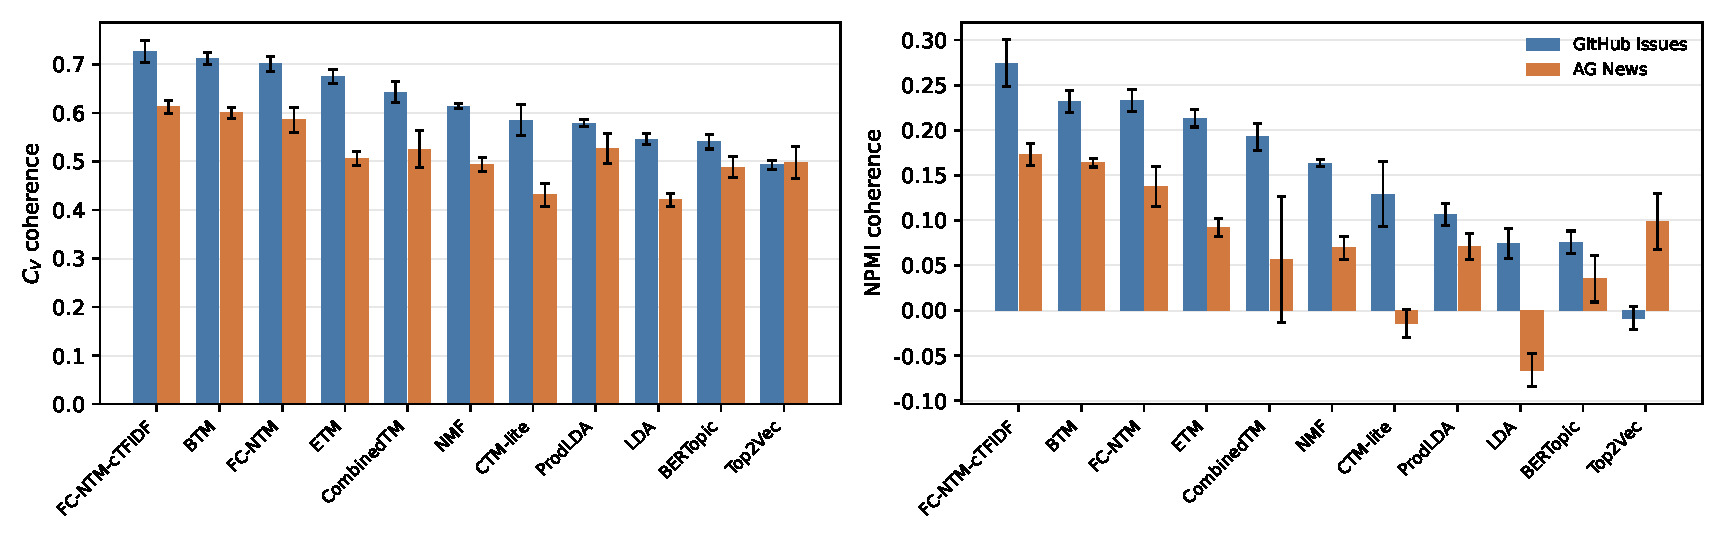
\includegraphics[width=0.86\textwidth]{fig_main_comparison_en.pdf}
\caption{Main results on the two public corpora (unified evaluation vocabulary, ten words per
topic). Left: $C_V$; right: NPMI. Error bars are standard deviations across seeds. The \fcntm{}
rows, BTM and ETM on GitHub and the \fcntm{} rows on AG News are three-seed results; CombinedTM,
ProdLDA and CTM-lite were run for the same seeds 11/23/37 under the same protocol.}
\label{fig:main}
\end{figure}

\begin{figure}[t]
\centering
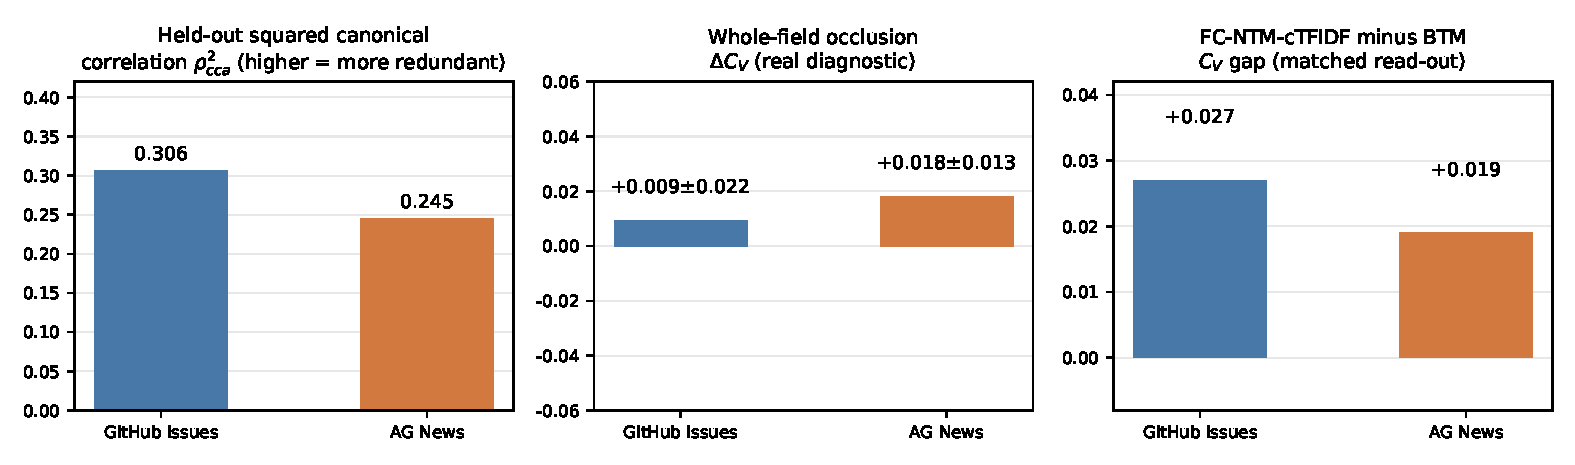
\includegraphics[width=0.86\textwidth]{fig_complementarity_en.pdf}
\caption{Field redundancy and gain (held-out measures). Left: squared canonical correlation $\rho^2_{\mathrm{cca}}$ (higher means more redundant; fitted on the training split and evaluated on the test split); middle: the $\Delta C_V$ of the real occlusion diagnostic (GitHub $+0.009\pm0.022$, AG News $+0.018\pm0.013$, three seeds each); right: the $C_V$ difference between \fcntm{}-cTFIDF and BTM under the matched read-out (GitHub $+0.027$, AG News $+0.019$). The two corpora have similar redundancy, while the ten-seed gain is positive on GitHub only (AG News $-0.009$), so the figure does not support a redundancy-based prediction of the gain.}\label{fig:cond}
\end{figure}

\begin{figure}[t]
\centering
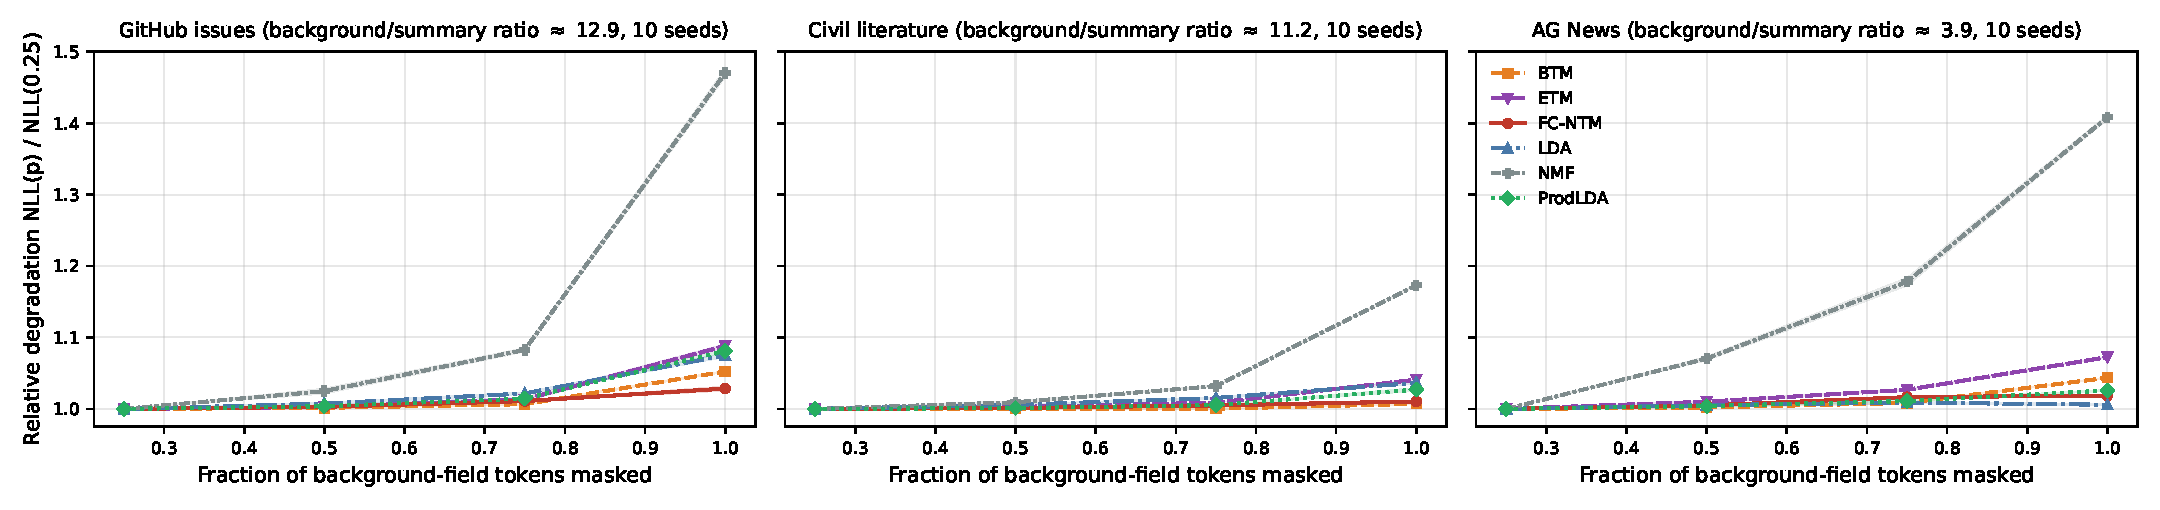
\includegraphics[width=0.86\textwidth]{fig_occlusion_cross_corpus_en.pdf}
\caption{Relative degradation under the same partial-occlusion protocol on three corpora (curves
are means, shading is $\pm1$ standard deviation; line style and marker identify the models, so the
curves remain distinguishable in black-and-white print; \fcntm{}, BTM and LDA cover the ten seeds
11--139, the remaining baselines keep the archived seeds 11/23/37). Left: GitHub issues
(background to summary length ratio $\approx12.9$); middle: civil engineering corpus
($\approx11.2$); right: AG News ($\approx3.9$). Only on GitHub is the degradation of \fcntm{}
clearly below all baselines; on the civil corpus and AG News the smallest degradation belongs to
BTM and LDA respectively, and the gap to \fcntm{} is within 0.003--0.013.}
\label{fig:occl-cross}
\end{figure}

\section{Ablation and read-out details}

The paragraphs below accompany Tables S9--S12 and describe the ablations,
the fusion-weight sensitivity and the field-restricted read-out in full.

\subsection{Ablation: fusion reconstruction and gating}



The three-step ablation separates two questions: whether the fused mixture receives its own
reconstruction term, and whether fusion is averaged or gated. The fusion-reconstruction term is
effective, but only for the read-out that uses the fused posterior: adding it under mean fusion
raises the class TF--IDF $C_V$ and NPMI by 0.014 and 0.013 (3/3 seeds) while lowering the $\beta$
read-out by 0.013 and 0.021. Replacing mean fusion by a gate brings no further gain in this corpus
and protocol (class TF--IDF differences $-0.001$ and $-0.000$, 1/3 seeds; $\beta$ read-out
$-0.007$ and $-0.012$, 0/3). This conclusion has a precise boundary: without the fusion
reconstruction term the gate receives no gradient and the model degenerates exactly to mean fusion,
so the experiment cannot separate the value of the gate parameters from the value of the fusion
objective; we report the absence of an observed gain rather than claiming that a trained gate is
useless in general.

\subsection{Ablation: core components}



Four components are switched off one at a time. First, removing the JS consistency term causes no
consistent change in topic quality on any corpus or read-out (all six cells
$|\Delta C_V|\leq0.004$, none with a clear positive paired majority): in this
parameterisation the fused representation is trained by the fusion-reconstruction objective, not by
pulling the two posteriors together. Second, the observed effect of cross-field reconstruction
and word masking depends on the corpus: on GitHub, removing cross-field reconstruction even raises
the $\beta$ read-out by 0.021 (2/3 seeds) and costs only 0.005 in the class TF--IDF read-out, while
on AG News and the civil corpus both read-outs drop when either component is removed (cross-field
reconstruction $-0.011/-0.022$ and $-0.022/-0.019$; word masking $-0.026/-0.043$ and
$-0.010/-0.012$, with all class TF--IDF columns at 0/3). Third, whole-field dropout acts mostly on
the class TF--IDF read-out and is consistently beneficial on two of the three corpora only: it
lowers both read-outs on GitHub
and AG News but changes the $\beta$ read-out of the civil corpus by only $+0.001$ while lowering
its class TF--IDF read-out by 0.034. Fourth, field asymmetry does not explain the component-level
differences: the civil corpus has almost the same length ratio as GitHub (11.2 versus 12.9) yet
behaves like AG News (3.9). The scope of the ablation is also limited: it switches off the
per-stream cross-field reconstruction while the fused reconstruction term still rebuilds both
fields, so it does not cut all information flow between fields.

\subsection{Sensitivity to the fusion weight}



At $\lambda_f=0.25$ the class TF--IDF read-out is essentially the no-fusion result ($C_V$ 0.713
versus 0.714) while the $\beta$ read-out has already dropped by 0.024; between 0.5 and 1.0 the
class TF--IDF gain is stable (0.727 versus 0.723, NPMI 0.274 versus 0.277, differences below
0.005), and the $\beta$ penalty narrows from $-0.020$ to $-0.005$ relative to $\lambda_f=0$.
The value 0.5 used throughout is therefore a conservative compromise.

\subsection{Field-restricted read-out}



Field-restricted read-out truncates the topic words to one field's vocabulary and scores them
against that field's own test text. With the shared decoder, the background-view $C_V$ of
\fcntm{} stays close to its full-vocabulary $\beta$ read-out on all three corpora (0.697, 0.566
and 0.637 versus 0.701, 0.586 and 0.633), while the summary view is lower in absolute terms mainly
because a summary contains only 3--5 tokens and the reference corpus is very short, so that column
should be compared within the same protocol only. The cross-model comparison shows that the
read-out is not unique to a two-stream encoder: BTM is slightly better in the background view on
GitHub and AG News (0.710 versus 0.697 and 0.586 versus 0.566), \fcntm{} leads only on the civil
corpus (0.637 versus 0.600 for NMF), and in the summary view LDA and ProdLDA are above \fcntm{}
on all three corpora (0.486 and 0.438 versus 0.423 on AG News). We therefore treat the field view
as a descriptive read-out available to any model with a topic--word matrix, not as evidence of a
unique structural advantage.

\end{document}
